% ICCIT 2026 submission. IEEE conference template, A4 (ICCIT requires the A4 template).
% DOUBLE-BLIND: no author names, affiliations, addresses, or emails anywhere.
% Build: pdflatex main && bibtex main && pdflatex main && pdflatex main
\documentclass[conference,a4paper]{IEEEtran}
\IEEEoverridecommandlockouts
\usepackage{cite}
\usepackage{amsmath,amssymb,amsfonts}
\usepackage{graphicx}
\usepackage{textcomp}
\usepackage{xcolor}

\begin{document}

\title{Closing the Synthetic-to-Real Gap in Tiny Aerial Human Detection
with a Small Labeled Budget}

% Double-blind submission: author block anonymized per ICCIT 2026 guidelines.
\author{\IEEEauthorblockN{Anonymous Submission}
\IEEEauthorblockA{\textit{Paper ID assigned by CMT}}}

\maketitle

\begin{abstract}
Detectors that find people in aerial disaster imagery are usually trained and
tested on synthetic benchmarks, so how they behave on real footage stays
unknown until deployment. This paper measures that behavior and shows what a
small labeling budget does about it. A compact detector trained on the
composited C2A benchmark is first evaluated zero-shot on three kinds of real
footage: drone video recorded at three altitudes, campus scenes with partial
occlusion, and disaster frames sampled from public news video. The gap is
severe, falling from 0.844 AP50 on the synthetic benchmark to 0.335 on drone
video and 0.133 on real disaster frames. Fine-tuning on the synthetic training
set mixed with 248 labeled real frames, roughly one afternoon of assisted
annotation through an audited pipeline, closes most of that gap. One
19.6-million-parameter model then reaches 0.795 on drone video, 0.689 on campus
scenes, and 0.411 on disaster footage from the training events, while the
synthetic benchmark drops only 0.7 points and confidence calibration improves.
A disaster event held out from all training bounds the result: there the gain is
not statistically significant, so the budget buys adaptation to the target
footage rather than to disasters in general. The adapted model runs at about
115 frames per second on a single consumer GPU.
\end{abstract}

\begin{IEEEkeywords}
aerial human detection, search and rescue, synthetic-to-real transfer, tiny
object detection, UAV imagery, disaster response
\end{IEEEkeywords}

\section{Introduction}
When a flood or an earthquake strikes, the first hours decide how many people
are found alive. A drone can sweep a disaster site far faster than a ground
team, but the footage it returns is punishing to search by eye. A person seen
from altitude spans a few dozen pixels at best, and one sortie produces
thousands of frames. Detectors that flag those people automatically are
therefore studied with growing interest, most often on C2A \cite{nihal2024c2a},
a large semi-synthetic dataset that composites segmented human figures onto
real disaster backgrounds. Synthetic data solves the scale problem, because
real annotated disaster imagery is scarce. It leaves open the question that
decides whether such a detector is useful in the field. What does a model
trained on composited scenes actually do when it meets real footage?

This paper answers that question with measurements, then shows how far a small
labeling budget goes toward closing the gap it exposes. We start from a compact
C2A-trained detector and evaluate it zero-shot on three kinds of real imagery:
our own drone video recorded at three altitudes, campus scenes in which people
are partly hidden by trees, and disaster frames sampled from public news video
of a flood and a building collapse. The drop is severe. A model that reaches
0.844 AP50 on the synthetic benchmark falls to 0.335 on the drone test set and
0.133 on real disaster frames. We then fine-tune on a mixture of the synthetic
training split and 248 labeled real frames, about one afternoon of
segmentation-assisted annotation, and evaluate everything again.
Fig.~\ref{fig:teaser} summarizes the outcome: the drone score rises to 0.795,
the disaster score triples to 0.411, and the synthetic benchmark loses less
than one point, so a single model serves every domain at once.

\begin{figure}[htbp]
\centerline{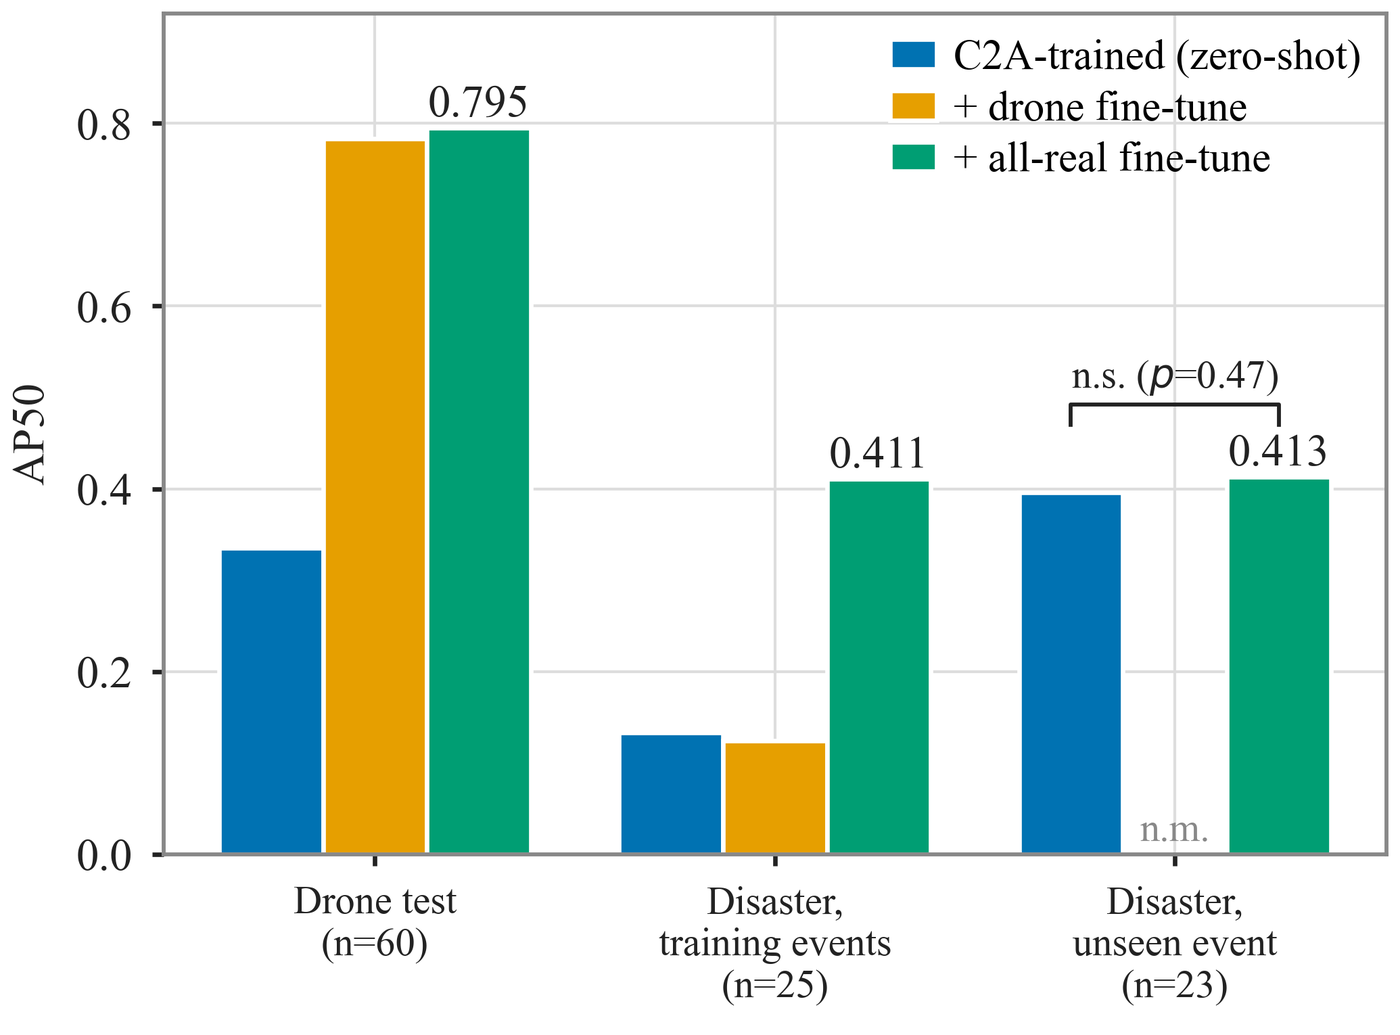
\includegraphics[width=\columnwidth]{figures/fig_adapt_stages_print.png}}
\caption{AP50 of three model stages on the three real evaluation domains.
Fine-tuning with 248 labeled real frames more than doubles the drone score and
triples the within-video disaster score. Drone-only fine-tuning leaves disaster
footage untouched (middle bars), so real-image exposure alone is not what
helps. On a disaster event held out from all training (right group) the adapted
and base models are statistically indistinguishable, which bounds how far this
budget generalizes.}
\label{fig:teaser}
\end{figure}

The study makes three contributions. The first is a multi-domain adaptation
result: one compact detector that holds 0.837 AP50 on C2A while reaching 0.795
on real drone footage, 0.689 on occluded campus scenes, and 0.411 on real
disaster frames, with calibration improving rather than degrading and no change
to parameter count or latency. The second is a low-cost pipeline for building
the real sets behind that result, from interval frame extraction and
perceptual-hash de-duplication through assisted annotation and automated label
audits, reproducible by any group with a consumer drone and public footage. The
third is a set of measured bounds: a held-out disaster event shows the
adaptation is specific to the footage it was trained on, so we report where the
budget stops paying as carefully as where it pays.

\section{Related Work}
Benchmarks for aerial person search fall into two groups. Real collections such
as SARD \cite{sambolek2021sard} and HERIDAL \cite{bozic2019heridal} contain
genuine search-and-rescue imagery, but only a few thousand frames, which is too
little to train a modern detector without heavy reliance on pretraining. C2A
\cite{nihal2024c2a} takes the opposite route. It composites segmented human
figures onto real disaster backgrounds drawn from aerial emergency imagery
\cite{kyrkou2020aider}, producing 10,215 images with roughly 360,000 instances,
most of them under 16 px. Published results on both kinds of dataset are almost
always in-domain: training and testing draw on the same distribution, so the
transfer question is left open. This paper measures it.

Transfer from synthetic training data has a longer history in robotics. Domain
randomization showed that models trained on varied synthetic scenes can work in
the real world \cite{tobin2017domainrand}, and Tremblay et al.
\cite{tremblay2018synthetic} showed that fine-tuning a synthetic-trained model
on a small amount of real data beats training on the real data alone. We adopt
that recipe, apply it to disaster person detection, and add the part the recipe
leaves out. A held-out event tests whether the adaptation reaches beyond the
footage it was tuned on.

Detecting people this small is a problem in its own right
\cite{cheng2023smallobject}. A stride-8 detection head summarizes an 8 by 8
pixel region in each cell, so people under ten pixels effectively vanish.
Common remedies add a stride-4 scale for drone imagery \cite{zhu2021tphyolov5},
re-weight features with attention such as CBAM \cite{woo2018cbam}, or slice the
input at inference time \cite{akyon2022sahi}. Our base detector already carries
modifications of this kind, and we hold it fixed. This study is about what data
does, not about what architecture does.

\section{Data and Method}
\label{sec:method}

\subsection{Base Detector}
The starting point is a YOLO11m \cite{jocher2024yolo11} variant built for tiny
aerial people. CBAM \cite{woo2018cbam} replaces the attention block at the end
of the backbone, a stride-4 detection scale extends the head to four levels,
and the task-aligned label assigner blends a normalized Wasserstein similarity
\cite{wang2021nwd} into its overlap term so that candidates for few-pixel
targets are ranked meaningfully. The model holds 19.6 million parameters and
86.7 GFLOPs, and it runs in 8.7 ms per image, about 115 frames per second, at
640 px input on a single consumer GPU. Training uses a scene-disjoint split of
C2A (6,135 training, 2,040 validation, and 2,040 test images) with AdamW at a
base learning rate of 0.001 for up to 300 epochs, and reaches 0.844 AP50 on the
C2A test set. Every experiment below holds this architecture fixed. Only the
training data changes.

\subsection{Real Imagery}
Three real training sets and five frozen evaluation sets were built for this
study. Table~\ref{tab:sets} lists them, and Fig.~\ref{fig:samples} shows one
sample from each source. The drone footage is our own 4K recording over open
ground at 10, 30, and 50 m altitude. The campus scenes come from the same
platform over a university campus at 30 and 50 m, where trees and buildings
hide parts of many people. The disaster frames were sampled from public news
video of two events, a flood and a building collapse. Frames from a third
event, unseen during any training, are reserved for evaluation only, and they
carry the weight of the generalization test in Section~\ref{sec:limits}. Median
person size runs from 44 px on the drone test set down to 17 px on the disaster
evaluation frames, so the real sets span the size regime that makes this task
hard.

\begin{table}[htbp]
\caption{Real-Imagery Sets Built for This Study}
\label{tab:sets}
\begin{center}
\begin{tabular}{|l|c|c|c|c|}
\hline
\textbf{Set} & \textbf{Role} & \textbf{Frames} & \textbf{Persons} & \textbf{Med. px} \\
\hline
Drone, 3 altitudes & train & 101 & 6,313 & --- \\
\hline
Drone, 3 altitudes & val & 14 & 973 & --- \\
\hline
Drone test & eval & 60 & 3,584 & 44 \\
\hline
Campus & train & 87 & 4,510 & 37 \\
\hline
Campus test & eval & 25 & 663 & 37 \\
\hline
Disaster, 2 events & train & 60 & 1,341 & 23 \\
\hline
Disaster, same events & eval & 25 & 1,070 & 17 \\
\hline
Disaster, unseen event & eval & 23 & 318 & 28 \\
\hline
\end{tabular}
\end{center}
\end{table}

\begin{figure*}[htbp]
\centerline{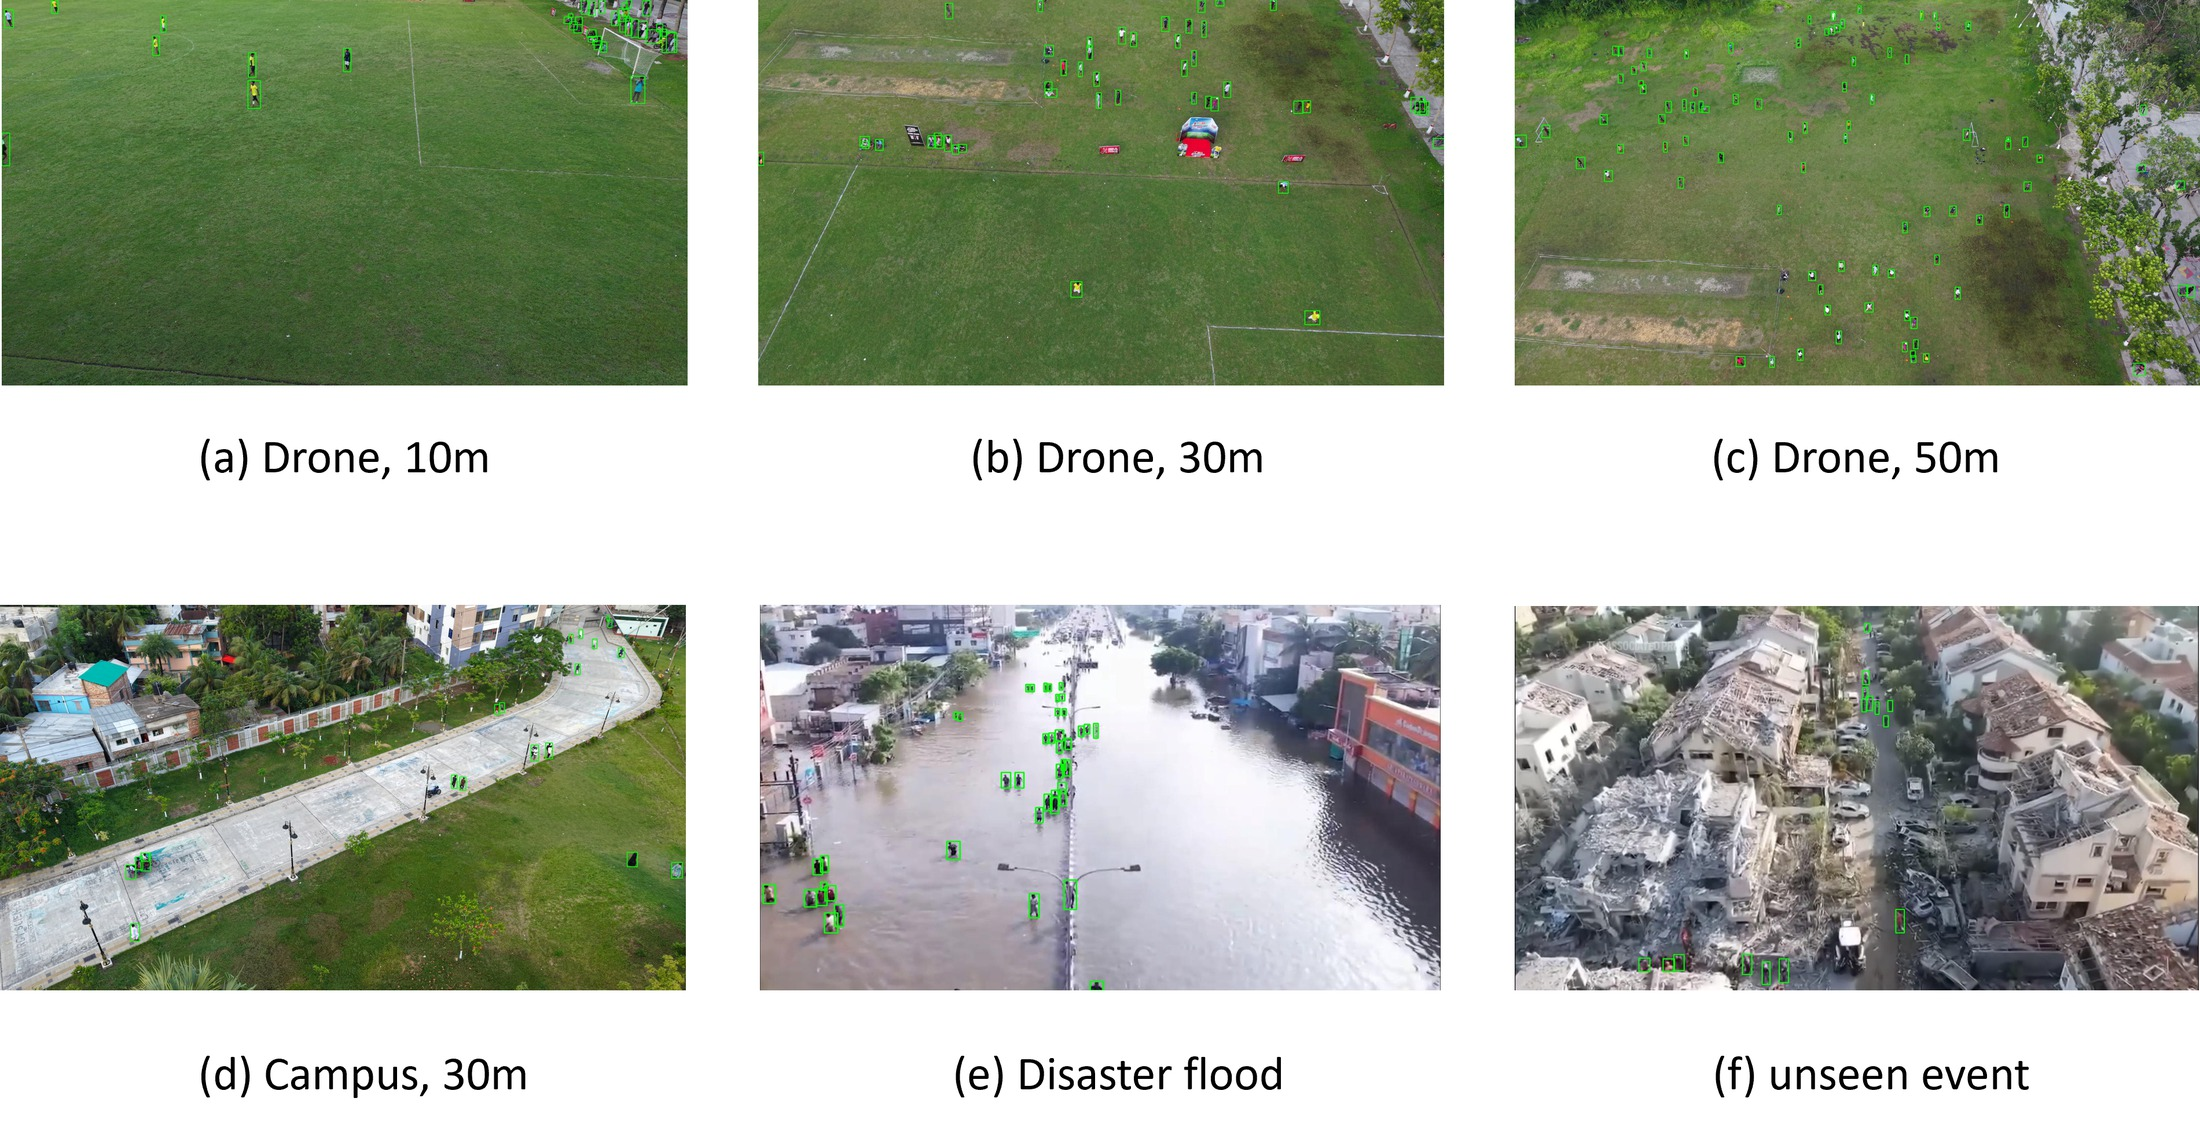
\includegraphics[width=0.86\textwidth]{figures/fig_real_samples.jpg}}
\caption{Samples from the real sets with ground-truth boxes. Panels (a) to (c)
show our drone footage at 10, 30, and 50 m altitude, where person size shrinks
with altitude; (d) is a campus scene in which trees hide parts of several
people; (e) is a flood frame from the disaster training videos; (f) is the
held-out unseen event. Disaster clutter and viewpoint differ from the
composited scenes the detector was trained on, and a large share of the
broadcast frame in (e) is taken up by black borders and station graphics.}
\label{fig:samples}
\end{figure*}

\subsection{Annotation Pipeline}
The pipeline behind these sets is deliberately cheap, because a rescue team
adapting a detector to its own region cannot afford a labeling campaign. Frames
are extracted from video at fixed intervals and de-duplicated with a perceptual
difference hash. The same hash is run against every evaluation frame, which
guarantees that no training frame is a near-duplicate of anything used for
testing. Annotation uses segmentation-assisted box drawing in a web tool: an
operator clicks a person, the tool proposes a mask, and the box follows. Every
visible person is boxed, and frames that contain no people are kept as explicit
negatives so the detector sees empty rubble and dark voids labeled as
background. An automated audit then rejects degenerate, duplicate, undersized,
and oversized boxes, and a visual overlay check of every frame closes the loop.
The complete disaster training set, 60 frames holding 1,341 people, took about
one afternoon.

\subsection{Adaptation Recipe and Evaluation Protocol}
Adaptation is a supervised fine-tune with no domain-adaptation machinery beyond
data mixing, which keeps the result a floor rather than a ceiling for more
elaborate methods. The training mixture holds the full C2A training split
together with the real training frames repeated twenty times, so that 248 real
frames are not drowned out by 6,135 synthetic images. The 4K frames are first
downscaled to 1,280 px on the long side, which keeps decoding and memory cost
manageable without touching the labels, since box coordinates are stored
relative to image size. The fine-tune runs at a reduced learning rate of
$5\times10^{-4}$ on a cosine schedule for at most 80 epochs, with early
stopping on both fitness and $F_2$; the selected model comes from epoch 66.

Evaluation reports AP50, the recall-weighted $F_2$ score that search and rescue
favors because a missed person costs more than a false alarm, recall at a fixed
0.25 operating threshold, and recall by target size in the bands very-tiny
(under 8 px), tiny (8 to 16 px), small (16 to 32 px), and medium (32 to 96 px),
measured as the square root of box area. Where two models are compared on the
same set, a paired image-level bootstrap over 1,000 resamples gives a 95\%
confidence interval and a two-sided $p$-value for the difference, so small gaps
on small sets are never over-read.

\section{Results}

\subsection{One Model, Five Held-Out Domains}
Table~\ref{tab:multi} is the central result. After fine-tuning on the mixed
set, one model is evaluated on every frozen test set, and no domain has to be
traded away for another. The synthetic benchmark barely moves, from 0.844 to
0.837 AP50, and its calibration improves rather than degrades: expected
calibration error falls from 0.014 to 0.011, so a reported confidence of 0.8
still corresponds to roughly 0.8 empirical precision and an operator can keep
trusting the scores. The drone test set rises from a zero-shot 0.335 to 0.795.
Campus scenes with partial occlusion, a domain that contributes only 87
training frames, reach 0.689. Real disaster footage from the training events
reaches 0.411, three times its zero-shot score. Parameter count, GFLOPs, and
latency are those of the base detector, unchanged, because only training data
was altered.

\begin{table}[htbp]
\caption{The Single Adapted Model on Every Held-Out Set}
\label{tab:multi}
\begin{center}
\begin{tabular}{|l|c|c|c|c|}
\hline
\textbf{Evaluation set} & \textbf{Images} & \textbf{AP50} & \textbf{$F_2$} & \textbf{Rec.$_{0.25}$} \\
\hline
C2A scene-disjoint test & 2,040 & 0.837 & 0.824 & 0.821 \\
\hline
Drone test & 60 & 0.795 & 0.771 & 0.837 \\
\hline
Campus & 25 & 0.689 & 0.666 & 0.718 \\
\hline
Disaster, training events & 25 & 0.411 & 0.472 & 0.451 \\
\hline
Disaster, unseen event & 23 & 0.413 & 0.451 & 0.374 \\
\hline
\end{tabular}
\end{center}
\end{table}

\subsection{What the Budget Buys, Domain by Domain}
The drone gap closes almost completely. Zero-shot, the C2A-trained model finds
a third of the people it should, with recall 0.337 at the operating threshold;
after adaptation it finds 0.837. AP50 climbs from 0.335 through 0.783 with
drone data alone to 0.795 with the full mixture, so the last 1.2 points come
from disaster and campus frames that share nothing with the drone domain except
being real. Disaster footage behaves differently, and Fig.~\ref{fig:teaser}
makes the contrast visible. Fine-tuning on drone footage alone does nothing for
disaster frames, moving them from 0.133 to 0.124, which is within noise. Sixty
labeled disaster frames are what help, and they help by a factor of three. The
gain arrives where the labels are, not where real images in general are.

\subsection{Where the Gains Land by Target Size}
Aggregate scores hide which people are actually being recovered, so
Table~\ref{tab:persize} breaks recall down by target size, each model measured
at its own optimal-$F_1$ threshold and bands without instances omitted. Two
patterns stand out. On the drone test set the gains are large in both bands that carry
instances, with small-object recall rising from 0.118 to 0.449 and medium
recall from 0.352 to 0.751. On the disaster evaluation set, where targets are
genuinely small, the 8 to 16 px band moves from 0.060 to 0.270 and the 16 to 32
px band from 0.230 to 0.569, better than a doubling in each case. The sub-8-px
band is the exception, and it does not move at all: recall there is zero before
adaptation and zero after it, across all 54 such instances. The smallest people
in real disaster scenes are not recovered by more data of this kind, which sets
a clear target for future work.

\begin{table}[htbp]
\caption{Recall by Target Size, Before and After Adaptation}
\label{tab:persize}
\begin{center}
\begin{tabular}{|l|c|c|c|c|}
\hline
\textbf{Set and band} & \textbf{Inst.} & \textbf{Zero-shot} & \textbf{Adapted} & \textbf{Change} \\
\hline
Drone, 16--32 px & 642 & 0.118 & 0.449 & $+0.331$ \\
\hline
Drone, 32--96 px & 2,826 & 0.352 & 0.751 & $+0.399$ \\
\hline
Disaster, under 8 px & 54 & 0.000 & 0.000 & $0.000$ \\
\hline
Disaster, 8--16 px & 433 & 0.060 & 0.270 & $+0.210$ \\
\hline
Disaster, 16--32 px & 427 & 0.230 & 0.569 & $+0.339$ \\
\hline
Disaster, 32--96 px & 154 & 0.370 & 0.688 & $+0.318$ \\
\hline
\end{tabular}
\end{center}
\end{table}

\subsection{Limits and Known Artifacts}
\label{sec:limits}
Three boundaries deserve to be stated plainly. First, the adaptation is
specific to the footage it saw. On the disaster event held out from all
training, the adapted model scores 0.413 AP50 against the base model's 0.396, a
difference of 1.7 points whose bootstrap interval spans zero ($[-3.2, 5.7]$,
$p = 0.47$), and precision at the operating threshold falls by 13.1 points
($p = 0.018$). Sixty frames from two events adapt the model to those events,
not to disasters in general. Second, as Table~\ref{tab:persize} shows, people
below 8 px in real disaster imagery remain undetected. Third, part of the
within-video gain rides on presentation artifacts rather than content: both
training clips are pillarboxed broadcast footage, in which 41\% and 47\% of
each frame is black border and station graphics, and the within-video
evaluation frames share that framing while the held-out clip does not. None of
this changes the deployment reading, since a rescue team adapting the detector
to its own region and platform sits squarely in the within-video regime. It
does say what the next step must be. Generalizing across unseen events will
need frames from many events rather than many frames from two, and the pipeline
of Section~
ef{sec:method} makes each additional event cheap to add.

\section{Conclusion}
A detector trained only on composited disaster scenes loses most of its skill on
real footage, and this paper measured both the loss and the cheapest known
repair. With 248 labeled real frames, roughly one afternoon of assisted
annotation, a 19.6-million-parameter model went from 0.335 to 0.795 AP50 on
real drone video and from 0.133 to 0.411 on real disaster frames, while the
synthetic benchmark it came from moved less than one point and its calibration
improved. Recall by size shows where those gains land, and where they do not:
people below 8 px in real disaster imagery stay invisible. The same experiment
also priced the limit of the budget, because a disaster event held out from
training gained nothing significant. For a rescue team the practical reading is
direct. Adapting this class of detector to the team's own region and platform
is an afternoon of work, while covering disasters in general remains a data
collection problem, one event at a time.

\bibliographystyle{IEEEtran}
\bibliography{references}

\end{document}
